\documentclass[border=10pt]{standalone}
\usepackage{tikz}
\usetikzlibrary{patterns}

\begin{document}
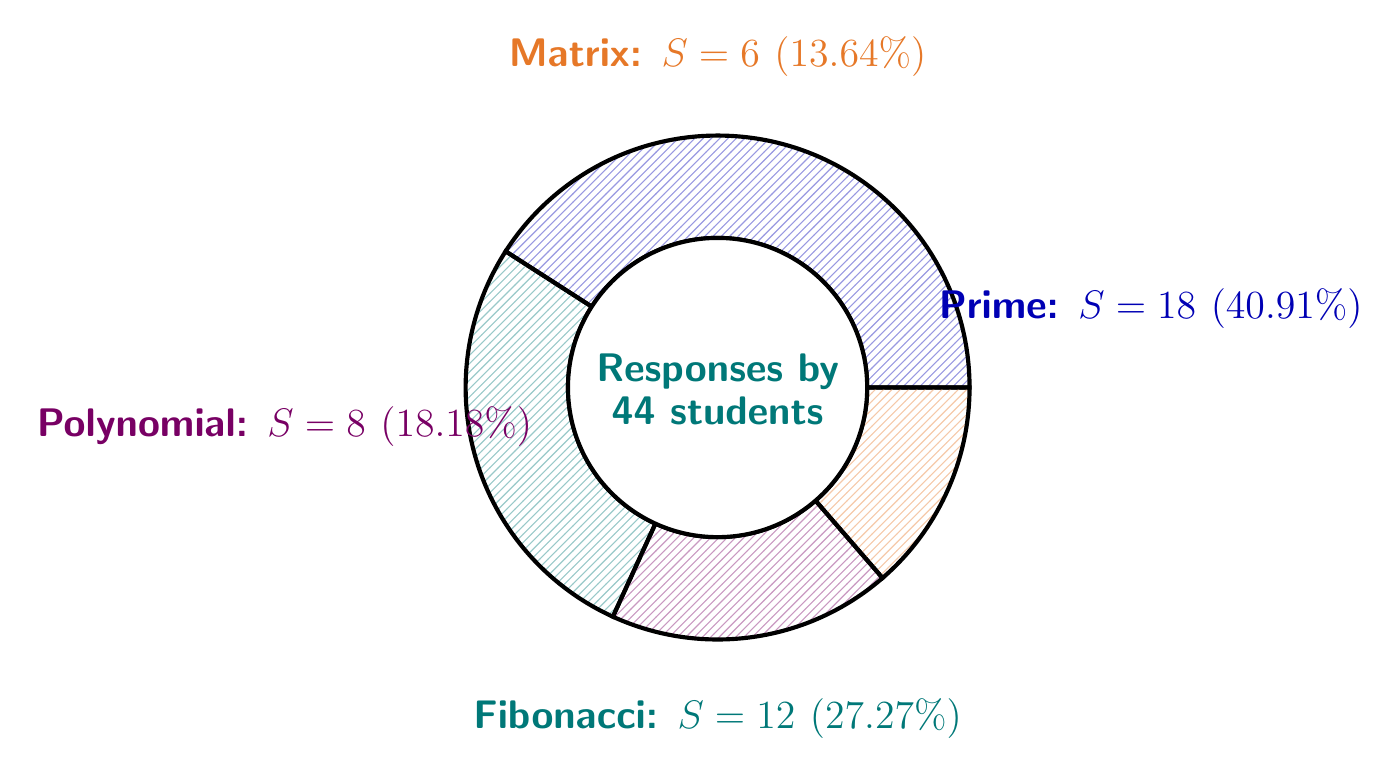
\begin{tikzpicture}[font=\sffamily\large]
    % Define colors
    \definecolor{primeblue}{RGB}{0,0,180}
    \definecolor{fibonacciteal}{RGB}{0,120,120}
    \definecolor{polynomialpurple}{RGB}{120,0,100}
    \definecolor{matrixorange}{RGB}{230,120,40}
    \definecolor{centertext}{RGB}{0,120,120}
    
    % Define parameters
    \def\outerradius{3.2}
    \def\innerradius{1.9}
    
    % Calculate angles (cumulative)
    % Prime: 40.91% -> 147.276 degrees
    % Fibonacci: 27.27% -> 98.172 degrees
    % Polynomial: 18.18% -> 65.448 degrees
    % Matrix: 13.64% -> 49.104 degrees
    
    \def\angleA{0}
    \def\angleB{147.276}
    \def\angleC{245.448}
    \def\angleD{310.896}
    
    % Draw segments with hatching
    % Prime segment (blue)
    \fill[primeblue, draw=black, line width=1.5pt, pattern=north east lines, pattern color=primeblue!40] 
        (\angleA:\outerradius) arc (\angleA:\angleB:\outerradius) 
        -- (\angleB:\innerradius) arc (\angleB:\angleA:\innerradius) -- cycle;
    
    % Fibonacci segment (teal)
    \fill[fibonacciteal, draw=black, line width=1.5pt, pattern=north east lines, pattern color=fibonacciteal!40] 
        (\angleB:\outerradius) arc (\angleB:\angleC:\outerradius) 
        -- (\angleC:\innerradius) arc (\angleC:\angleB:\innerradius) -- cycle;
    
    % Polynomial segment (purple)
    \fill[polynomialpurple, draw=black, line width=1.5pt, pattern=north east lines, pattern color=polynomialpurple!40] 
        (\angleC:\outerradius) arc (\angleC:\angleD:\outerradius) 
        -- (\angleD:\innerradius) arc (\angleD:\angleC:\innerradius) -- cycle;
    
    % Matrix segment (orange)
    \fill[matrixorange, draw=black, line width=1.5pt, pattern=north east lines, pattern color=matrixorange!40] 
        (\angleD:\outerradius) arc (\angleD:360:\outerradius) 
        -- (360:\innerradius) arc (360:\angleD:\innerradius) -- cycle;
    
    % Center white circle
    \fill[white, draw=black, line width=1.5pt] (0,0) circle (\innerradius);
    
    % Center text
    \node[centertext, align=center, font=\sffamily\Large\bfseries] at (0,0.2) {Responses by};
    \node[centertext, align=center, font=\sffamily\Large\bfseries] at (0,-0.3) {44 students};
    
    % Labels
    % Prime label (right)
    \node[primeblue, align=left, font=\sffamily\Large\bfseries] at (5.5,1) 
        {\textbf{Prime:} $S=18$ $(40.91\%)$};
    
    % Fibonacci label (bottom)
    \node[fibonacciteal, align=center, font=\sffamily\Large\bfseries] at (0,-4.2) 
        {\textbf{Fibonacci:} $S=12$ $(27.27\%)$};
    
    % Polynomial label (left)
    \node[polynomialpurple, align=right, font=\sffamily\Large\bfseries] at (-5.5,-0.5) 
        {\textbf{Polynomial:} $S=8$ $(18.18\%)$};
    
    % Matrix label (top)
    \node[matrixorange, align=center, font=\sffamily\Large\bfseries] at (0,4.2) 
        {\textbf{Matrix:} $S=6$ $(13.64\%)$};
    
\end{tikzpicture}
\end{document}